\documentclass[12pt]{article}
\usepackage[utf8]{inputenc}
\usepackage{booktabs}
\usepackage{geometry}
\usepackage{graphicx}
\geometry{a4paper, margin=1in}
\title{Results of the Fisher Combined Test}
\author{Sara Fraija}
\date{\today}
\begin{document}
\maketitle
\section{Resultados}

\begin{table}[h!]
\centering
\resizebox{\textwidth}{!}{%
\begin{tabular}{l c c c c c c}
\toprule
\textbf{GRB} & \textbf{Transit} & \textbf{Significance} & \textbf{Significance Corregida} & \textbf{p-value} & \textbf{Corrected p-value} & \textbf{PDF} \\ \midrule
GRB170708046 & 1__plus_20 & 0.97 & 0.26 & 8.340e-01 & 3.961e-01 & 7.508e-01 \\
GRB170816599 & 1__plus_20 & 2.29 & 1.88 & 9.890e-01 & 3.029e-02 & 9.710e-01 \\
GRB170222209 & 1__plus_20 & 2.13 & 1.22 & 9.834e-01 & 1.121e-01 & 9.587e-01 \\
GRB170403583 & 1__plus_20 & 0.00 & -2.00 & 5.000e-01 & 9.770e-01 & 6.011e-01 \\
GRB170826369 & 1__plus_20 & 0.00 & -2.69 & 5.000e-01 & 9.965e-01 & 6.011e-01 \\
GRB190515190 & 1__plus_20 & 2.26 & 1.26 & 9.881e-01 & 1.037e-01 & 9.690e-01 \\
GRB150101270 & 1__plus_20 & 1.49 & 1.49 & 9.319e-01 & 6.811e-02 & 8.685e-01 \\
GRB150101641 & 1__plus_20 & 1.64 & 1.64 & 9.495e-01 & 5.050e-02 & 8.960e-01 \\
GRB150110923 & 1__plus_20 & 1.02 & 1.02 & 8.461e-01 & 1.539e-01 & 7.629e-01 \\
GRB150120123 & 1__plus_20 & 1.88 & 1.88 & 9.699e-01 & 3.005e-02 & 9.319e-01 \\
GRB150922234 & 1__plus_20 & 1.09 & 1.09 & 8.621e-01 & 1.379e-01 & 7.797e-01 \\
GRB151228129 & 1__plus_20 & 1.80 & 1.80 & 9.641e-01 & 3.593e-02 & 9.210e-01 \\
GRB151229285 & 1__plus_20 & 3.18 & 3.18 & 9.993e-01 & 7.364e-04 & 9.975e-01 \\
GRB160612842 & 1__plus_20 & 0.00 & -0.00 & 5.000e-01 & 5.000e-01 & 6.011e-01 \\
GRB160624477 & 1__plus_20 & 1.70 & 1.70 & 9.554e-01 & 4.457e-02 & 9.060e-01 \\
GRB160726065 & 1__plus_20 & 2.80 & 2.80 & 9.974e-01 & 2.555e-03 & 9.921e-01 \\
GRB170318644 & 1__plus_20 & 0.73 & 0.73 & 7.673e-01 & 2.327e-01 & 6.944e-01 \\
GRB170325331 & 1__plus_20 & 0.00 & -0.00 & 5.000e-01 & 5.000e-01 & 6.011e-01 \\
GRB170803729 & 1__plus_20 & 1.48 & 1.48 & 9.306e-01 & 6.944e-02 & 8.666e-01 \\
GRB170817529 & 1__plus_20 & 1.15 & 1.15 & 8.749e-01 & 1.251e-01 & 7.941e-01 \\
GRB180204109 & 1__plus_20 & 2.18 & 2.18 & 9.854e-01 & 1.463e-02 & 9.629e-01 \\
GRB180418281 & 1__plus_20 & 1.76 & 1.76 & 9.608e-01 & 3.920e-02 & 9.152e-01 \\
GRB180715755 & 1__plus_20 & 1.30 & 1.30 & 9.032e-01 & 9.680e-02 & 8.286e-01 \\
GRB180718082 & 1__plus_20 & 0.43 & 0.43 & 6.664e-01 & 3.336e-01 & 6.363e-01 \\
GRB180805543 & 1__plus_20 & 0.92 & 0.92 & 8.212e-01 & 1.788e-01 & 7.387e-01 \\
GRB181125371 & 1__plus_20 & 1.41 & 1.41 & 9.207e-01 & 7.927e-02 & 8.524e-01 \\
GRB190427190 & 1__plus_20 & 1.04 & 1.04 & 8.508e-01 & 1.492e-01 & 7.677e-01 \\
GRB201008443 & 1__plus_20 & 1.06 & 1.06 & 8.554e-01 & 1.446e-01 & 7.725e-01 \\
GRB201214672 & 1__plus_20 & 1.14 & 1.14 & 8.729e-01 & 1.271e-01 & 7.917e-01 \\
GRB210323918 & 1__plus_20 & 1.34 & 1.34 & 9.099e-01 & 9.012e-02 & 8.374e-01 \\
GRB211024065 & 1__plus_20 & 0.10 & 0.10 & 5.398e-01 & 4.602e-01 & 6.030e-01 \\
GRB220412713 & 1__plus_20 & 1.38 & 1.38 & 9.162e-01 & 8.379e-02 & 8.461e-01 \\
GRB220418720 & 1__plus_20 & 0.40 & 0.40 & 6.554e-01 & 3.446e-01 & 6.317e-01 \\
GRB220511571 & 1__plus_20 & 0.91 & 0.91 & 8.186e-01 & 1.814e-01 & 7.363e-01 \\
GRB220617772 & 1__plus_20 & 0.46 & 0.46 & 6.772e-01 & 3.228e-01 & 6.411e-01 \\
GRB221120895 & 1__plus_20 & 0.00 & -0.00 & 5.000e-01 & 5.000e-01 & 6.011e-01 \\
GRB230228244 & 1__plus_20 & 0.00 & -0.00 & 5.000e-01 & 5.000e-01 & 6.011e-01 \\
GRB230512269 & 1__plus_20 & 0.09 & 0.09 & 5.359e-01 & 4.641e-01 & 6.027e-01 \\
GRB230812790 & 1__plus_20 & 0.00 & -0.00 & 5.000e-01 & 5.000e-01 & 6.011e-01 \\
GRB150819440 & 2__plus_20 & 1.37 & 0.77 & 9.147e-01 & 2.195e-01 & 8.439e-01 \\
GRB170708046 & 2__plus_20 & 0.68 & -0.12 & 7.517e-01 & 5.474e-01 & 6.834e-01 \\
GRB170816599 & 2__plus_20 & 2.69 & 2.33 & 9.964e-01 & 9.892e-03 & 9.893e-01 \\
GRB170206453 & 2__plus_20 & 0.68 & -1.27 & 7.517e-01 & 8.988e-01 & 6.834e-01 \\
GRB170222209 & 2__plus_20 & 0.82 & -0.86 & 7.939e-01 & 8.063e-01 & 7.150e-01 \\
GRB170403583 & 2__plus_20 & 0.00 & -2.00 & 5.000e-01 & 9.770e-01 & 6.011e-01 \\
GRB170826369 & 2__plus_20 & 0.26 & -2.14 & 6.026e-01 & 9.838e-01 & 6.143e-01 \\
GRB190515190 & 2__plus_20 & 0.47 & -1.88 & 6.808e-01 & 9.702e-01 & 6.428e-01 \\
GRB141205337 & 2__plus_20 & 1.01 & 1.01 & 8.438e-01 & 1.562e-01 & 7.604e-01 \\
GRB150101270 & 2__plus_20 & 0.40 & 0.40 & 6.554e-01 & 3.446e-01 & 6.317e-01 \\
GRB150101641 & 2__plus_20 & 0.45 & 0.45 & 6.736e-01 & 3.264e-01 & 6.395e-01 \\
GRB150922234 & 2__plus_20 & 0.98 & 0.98 & 8.365e-01 & 1.635e-01 & 7.532e-01 \\
GRB151229285 & 2__plus_20 & 0.00 & -0.00 & 5.000e-01 & 5.000e-01 & 6.011e-01 \\
GRB160612842 & 2__plus_20 & 0.00 & -0.00 & 5.000e-01 & 5.000e-01 & 6.011e-01 \\
GRB160624477 & 2__plus_20 & 2.00 & 2.00 & 9.772e-01 & 2.275e-02 & 9.460e-01 \\
GRB160726065 & 2__plus_20 & 2.26 & 2.26 & 9.881e-01 & 1.191e-02 & 9.690e-01 \\
GRB170318644 & 2__plus_20 & 2.20 & 2.20 & 9.861e-01 & 1.390e-02 & 9.645e-01 \\
GRB170325331 & 2__plus_20 & 0.22 & 0.22 & 5.871e-01 & 4.129e-01 & 6.106e-01 \\
GRB170803729 & 2__plus_20 & 0.00 & -0.00 & 5.000e-01 & 5.000e-01 & 6.011e-01 \\
GRB170817529 & 2__plus_20 & 0.57 & 0.57 & 7.157e-01 & 2.843e-01 & 6.609e-01 \\
GRB171007498 & 2__plus_20 & 0.00 & -0.00 & 5.000e-01 & 5.000e-01 & 6.011e-01 \\
GRB180204109 & 2__plus_20 & 0.89 & 0.89 & 8.133e-01 & 1.867e-01 & 7.315e-01 \\
GRB180402406 & 2__plus_20 & 1.53 & 1.53 & 9.370e-01 & 6.301e-02 & 8.762e-01 \\
GRB180418281 & 2__plus_20 & 1.26 & 1.26 & 8.962e-01 & 1.038e-01 & 8.196e-01 \\
GRB180715755 & 2__plus_20 & 0.00 & -0.00 & 5.000e-01 & 5.000e-01 & 6.011e-01 \\
GRB180718082 & 2__plus_20 & 0.00 & -0.00 & 5.000e-01 & 5.000e-01 & 6.011e-01 \\
GRB180805543 & 2__plus_20 & 0.00 & -0.00 & 5.000e-01 & 5.000e-01 & 6.011e-01 \\
GRB181125371 & 2__plus_20 & 0.45 & 0.45 & 6.736e-01 & 3.264e-01 & 6.395e-01 \\
GRB190427190 & 2__plus_20 & 0.00 & -0.00 & 5.000e-01 & 5.000e-01 & 6.011e-01 \\
GRB200415367 & 2__plus_20 & 0.82 & 0.82 & 7.939e-01 & 2.061e-01 & 7.150e-01 \\
GRB201008443 & 2__plus_20 & 0.03 & 0.03 & 5.120e-01 & 4.880e-01 & 6.012e-01 \\
GRB201214672 & 2__plus_20 & 2.07 & 2.07 & 9.808e-01 & 1.923e-02 & 9.532e-01 \\
GRB210323918 & 2__plus_20 & 0.71 & 0.71 & 7.611e-01 & 2.389e-01 & 6.899e-01 \\
GRB210618072 & 2__plus_20 & 1.47 & 1.47 & 9.292e-01 & 7.078e-02 & 8.646e-01 \\
GRB220412713 & 2__plus_20 & 0.42 & 0.42 & 6.628e-01 & 3.372e-01 & 6.347e-01 \\
GRB220418720 & 2__plus_20 & 2.04 & 2.04 & 9.793e-01 & 2.068e-02 & 9.502e-01 \\
GRB220511571 & 2__plus_20 & 0.46 & 0.46 & 6.772e-01 & 3.228e-01 & 6.411e-01 \\
GRB220617772 & 2__plus_20 & 2.02 & 2.02 & 9.783e-01 & 2.169e-02 & 9.481e-01 \\
GRB221120895 & 2__plus_20 & 0.00 & -0.00 & 5.000e-01 & 5.000e-01 & 6.011e-01 \\
GRB230228244 & 2__plus_20 & 0.00 & -0.00 & 5.000e-01 & 5.000e-01 & 6.011e-01 \\
GRB230512269 & 2__plus_20 & 0.56 & 0.56 & 7.123e-01 & 2.877e-01 & 6.590e-01 \\
GRB230812790 & 2__plus_20 & 0.00 & -0.00 & 5.000e-01 & 5.000e-01 & 6.011e-01 \\
\bottomrule
\end{tabular}%
}
\caption{Lista de GRBs with sus Transits, Significances, Significances Corregidas, p-values, p-values Corregidos y valores PDF.}
\end{table}

\begin{figure}[h!]
\centering
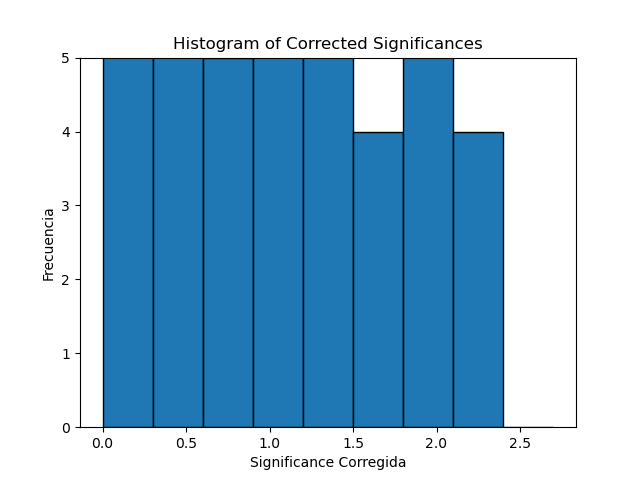
\includegraphics[width=0.6\textwidth]{corrected_significance_hist.png}
\caption{Histogram of Corrected Significances.}
\end{figure}

\section*{Conclusion}
The Fisher combined test integrates individual p-values to evaluate a global hypothesis.
The resulting test statistic was $X^2 = 294.347$ with 162 degrees of freedom.
For a significance level of 0.05, the critical value is 192.700.
Since $X^2$ is greater than the critical value, we rechazamos the null hypothesis of independence.
Normal approximation: p-value = 1.090e-09, significance ≈ 5.98 sigma.

\end{document}